\section{Lossy shortcuts and their price}
\label{sec:lossy}

\begin{figure*}[t]
\centering
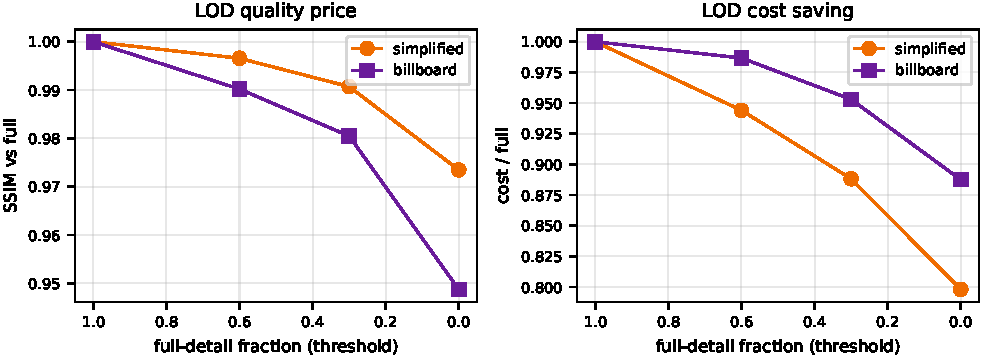
\includegraphics[width=\textwidth]{figures/lod_curve.pdf}
\caption{Level of detail. Left: SSIM against the full-detail image as more of
the field is simplified (threshold decreasing to the right). Right: the matching
cost fraction. Billboards are cheaper but degrade quality faster than the
single-triangle simplification.}
\label{fig:lod}
\end{figure*}

\begin{figure*}[t]
\centering
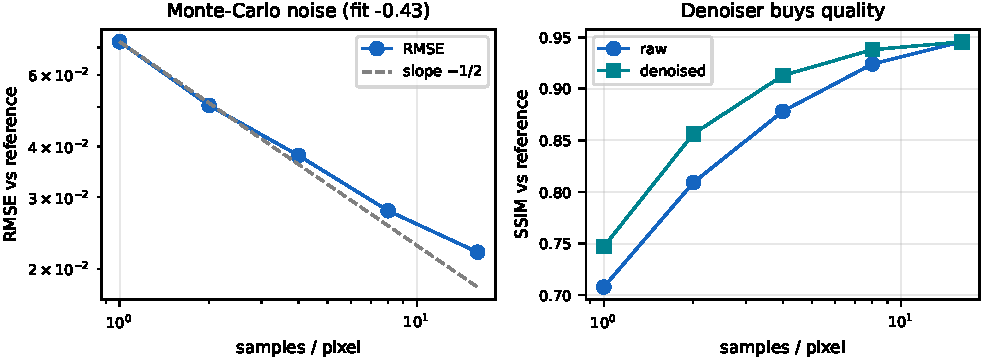
\includegraphics[width=\textwidth]{figures/sampling.pdf}
\caption{Sample budget. Left: RMSE against the reference versus samples per
pixel, tracking the theoretical $N^{-1/2}$ slope (fit \McSlope). Right: SSIM
with and without the guided denoiser --- the denoiser helps most where noise is
worst, at low sample counts.}
\label{fig:sampling}
\end{figure*}

Unlike Section~\ref{sec:accel}, the next two techniques change the image, so the
question becomes how much quality each unit of saved cost costs.

\paragraph{Level of detail.} Figure~\ref{fig:lod} sweeps the distance threshold
from all-full to all-simplified. Collapsing every far blade to a single triangle
holds SSIM at \LodSimpFloor\ --- a barely perceptible change --- while the flat
billboard, cheaper still, falls to \LodBillFloor. The striking part is the cost
axis: the saving is modest (down to \LodCostFloor\% of full-detail cost), far
smaller than the geometry reduction. The reason is precisely the previous
section: once a BVH is in place, halving the triangle count barely moves
traversal cost, because most of that cost is boxes, not triangles. LOD's classic
payoff --- fewer triangles to store, transform, and rasterise --- is a memory and
front-end win; inside a ray tracer with a good BVH, it is a weak lever on
intersection cost. That is a result worth stating plainly, and it reframes when
LOD is and is not the right tool.

\paragraph{Sample budget and denoising.} The stochastic side behaves as theory
predicts: Figure~\ref{fig:sampling} (left) shows RMSE falling with the
$N^{-1/2}$ Monte-Carlo slope (measured \McSlope), so quality here is bought by
brute-force sampling at a punishing exchange rate. The denoiser changes the
rate. At one sample per pixel it lifts SSIM from \SsimOneSpp\ to \SsimOneSppDn\
(a \DenoiseGainOne-point gain) by exploiting the noise-free G-buffer to smooth
within surfaces without crossing edges; the benefit shrinks as samples rise and
the image is already clean, exactly as it should. A cheap spatial filter guided
by geometry is worth several times its cost in samples in the noisy regime ---
the principle, in miniature, behind production denoisers.
